\chapter{Kravspecifikation}

\section{Funktionelle krav}
De funktionelle krav vil nedenstående beskrives ud fra aktør-kontekstdiagram, aktørbeskrivelse, Use Cases samt Use Case diagram. 

\subsection{Aktør-kontekstdiagram}

\begin{figure}[htb]
	\centering
	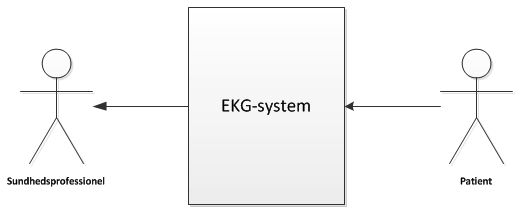
\includegraphics[width=1\textwidth]{Figurer/Snip20150226_1}
	\caption{Aktør-kontekstdiagram}
	\label{fig:aktoerbeskrivelse}
\end{figure}

\subsection{Aktørbeskrivelse}

\begin{table}[H]
\begin{tabularx}{\textwidth}{l l X}
    \toprule
     Aktørnavn  & Type      & Beskrivelse \\ \midrule
     Sundhedsprofessionelle   & Primær    & Det er den sundhedsproffesionelle, der ønsker at foretage EKG-målinger samt analysere på EKG-grafen.\\ 						  									  \addlinespace[2mm]
     Patienten & Sekundær  & Patienten sender elektroniske signaler til EKG-systemet, via elektroder, som er placeret på patientens krop\\                                                                                                                                                                            
   
     \bottomrule                                                                                                                   
    \end{tabularx}
    \caption {Aktørbeskrivelse}
    \label{tab:aktoerbeskrivelse}
	
\end{table}

Selve EKG-systemet består af tre elektroder, en EKG-forstærker, en NI 6009 DAQ og Visual studio. De tre elektroder skal fastgøres på patientens krop i forhold til afledning II. Elektroderne er koblet til EKG-forstærkeren som igen er koblet sammen med DAQ'en. DAQ'en er koblet til computeren via en USB-port. Selve programmet kører i Visual studio, hvor EKG-dataerne bliver behandlet og EKG-signalet vises som en graf. 

\subsection{Use Cases}

\begin{table}[H] % UC1 % 
    \begin{tabularx}{\textwidth}{l X}
    \toprule 
    \multicolumn{2}{c}{\begin{large}\textbf{Use Case 1}\end{large}}
 \\ \midrule \addlinespace[1mm]                                                                                                                                                        
     Navn:                  &  Vis EKG. \\ \addlinespace[1mm]                                                                                                                                                       
     Use Case ID:           & 1                                                                                                                                                                                                                                                                                                                                                                                                                                                                                                                                                                                                                         \\ \addlinespace[1mm]                                                                                                                                                       
     Samtidige forekomster: & 1                                                                                                                                                                                                                                                                                                                                                                                                                                                                                                                                                                                                                         \\ \addlinespace[1mm]                                                                                                                                                       
     Primær aktør:          &	Sundhedsprofessionelle.                                                                                                                                                                                                                                                                                                                                                                                                                                                                                                                                                                                                                 \\ \addlinespace[1mm] 
     Sekundær aktør:        &	Patienten                                                                                                                                                                                                                                                                                                                                                                                                                                                                                                                                                                                                                 \\ \addlinespace[1mm]  		                                                                                                                                                      
     Initialisere:          & 	Den sundhedsprofessionelle ønsker at få vist et EKG-signal over patienten.
		 \\ \addlinespace[1mm]                                                                                                                                                                                                                                                                                                             
     Forudsætninger:        & 	EKG-elektroder er koblet rigtigt op på patienten ud fra afledning II
     \begin{itemize}
     	\item Rød(+) på venstre ben
     	\item Sort(-) på højre arm
     	\item Grøn på venstre arm
     \end{itemize}
		Samt EKG-systemet er tændt og klar til måling.                                                                                                                                                                                                                                                                                                                                                                                                                                                                                                                                                                           \\ \addlinespace[1mm]                                                                                                                                                       
     Resultat:              & 	Den sundhedsprofessionelle kan ud fra EKG-dataerne se en graf.                                                                                                                                                                                                                                                                                                                                                                                                                                                                                                                                                   \\ \midrule \addlinespace[1mm]                                                                                                                                                       
     Hovedforløb:           &  \begin{enumerate}
     						   \item Elektroderne placeres på patientens krop ud fra afledning II
     						   
     						   \begin{itemize}
     						   	\item Rød(+) på venstre ben 
     						   	\item Sort(-) på højre arm 
     						   	\item Grøn på venstre arm
     						   \end{itemize}

     						   \item Den sundhedsprofessionelle vælger tidsindstillinger
\newline						[Extension 2a: Den sundhedsprofessioneller er tilfreds med default-indstillingerne]
     						   \item Målingen startes ved at trykke på "Start"
		   				   	   \item EKG-dataerne illustreres på en graf
     						   \end{enumerate}
\\ \midrule 
 	Undtagelser:           & \textit{Extensions:}
\newline					 2a: Der blev ikke ændret i tidsindstillingerne. 
\\ \bottomrule
    \end{tabularx}
    \caption {Fullydressed Use Case beskrivelse af UC1.}
    \label{tab:UC1}
\end{table}




\begin{table}[H] % UC2 % 
    \begin{tabularx}{\textwidth}{l X}
    \toprule 
    \multicolumn{2}{c}{\begin{large}\textbf{Use Case 2}\end{large}}
 \\ \midrule \addlinespace[1mm]                                                                                                                                                        
     Navn:                  &  Evaluer EKG i forhold til HRV. \\ \addlinespace[1mm]                                                                                                                                                       
     Use Case ID:           & 2                                                                                                                                                                                                                                                                                                                                                                                                                                                                                                                                                                                                                         \\ \addlinespace[1mm]                                                                                                                                                       
     Samtidige forekomster: & 1                                                                                                                                                                                                                                                                                                                                                                                                                                                                                                                                                                                                                         \\ \addlinespace[1mm]                                                                                                                                                       
     Primær aktør:          &	Sundhedsprofessionelle.                                                                                                                                                                                                                                                                                                                                                                                                                                                                                                                                                                                                                 \\ \addlinespace[1mm] 	                                                                                                                                                      
     Initialisere:          & 	At kunne evaluere variationen i længden af RR-intervaller.
		 \\ \addlinespace[1mm]                                                                                                                                                                                                                                                                                                             
     Forudsætninger:        & 	Use Case 1 er gennemført.                                                                                                                                                                                                                                                                                                                                                                                                                                                                                                                                                                           \\ \addlinespace[1mm]                                                                                                                                                       
     Resultat:              & 	HRV kan ses ud fra grafen.                                                                                                                                                                                                                                                                                                                                                                                                                                                                                                                          \\ \midrule \addlinespace[1mm]                                                                                                                                                       
     Hovedforløb:           &  \begin{enumerate}
     						   \item Den sundhedsprofessionelle måler længden mellem RR-intervallerne.
     						   \item Den sundhedsprofessionelle analysere målingerne
     						   \item HRV er identificeret
\newline						[Extensions 3a: HRV er ikke identificerbart]
     						   \end{enumerate}
\\ \midrule 
 	Undtagelser:           & \textit{Extensions:}
\newline					 3a: Det er er ikke mulig at analysere HRV ud fra grafen. 
\\ \bottomrule
    \end{tabularx}
    \caption {Fullydressed Use Case beskrivelse af UC2.}
    \label{tab:UC2}
\end{table}

\subsection{Use case-diagram}

\begin{figure}[htb]
	\centering
	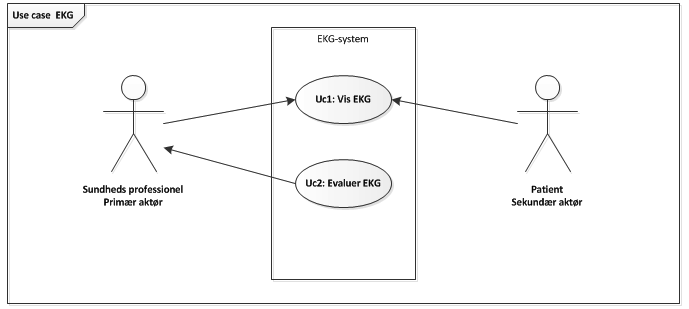
\includegraphics[width=1\textwidth]{Figurer/Snip20150226_2}
	\caption{Use case-diagram}
	\label{fig:Use Cases}
\end{figure}


















